%! \usetikzlibrary{decorations.pathreplacing,decorations.pathmorphing}
\usetikzlibrary{decorations.pathmorphing,decorations.markings}
\providecommand{\ket}[1]{\left|#1\right\rangle}
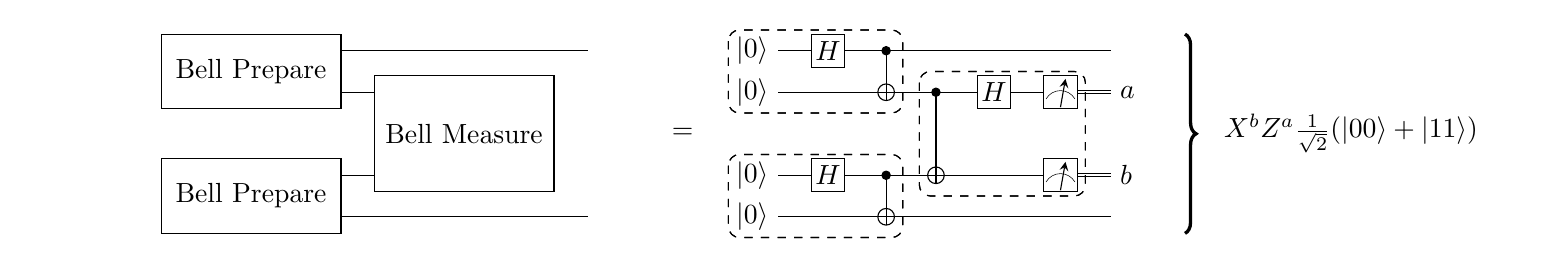
\begin{tikzpicture}[scale=1.000000,x=1pt,y=1pt]
\filldraw[color=white] (0.000000, -7.500000) rectangle (544.000000, 67.500000);
% Drawing wires
% Line 11: x W {} {} {\ket{0}} {}
\draw[color=white] (21.000000,60.000000) -- (80.500000,60.000000);
\draw[color=black] (80.500000,60.000000) -- (209.500000,60.000000);
\draw[color=black] (263.500000,60.000000) -- (398.500000,60.000000);
% Line 12: y W {} {} {\ket{0}} {a}
\draw[color=white] (21.000000,45.000000) -- (80.500000,45.000000);
\draw[color=black] (80.500000,45.000000) -- (157.500000,45.000000);
\draw[color=white] (157.500000,45.000000) -- (209.500000,45.000000);
\draw[color=black] (263.500000,45.000000) -- (373.000000,45.000000);
\draw[color=black] (373.000000,44.500000) -- (398.500000,44.500000);
\draw[color=black] (373.000000,45.500000) -- (398.500000,45.500000);
% Line 13: buf W
\draw[color=white] (13.500000,30.000000) -- (28.500000,30.000000);
% Line 14: z W {} {} {\ket{0}} {b}
\draw[color=white] (21.000000,15.000000) -- (80.500000,15.000000);
\draw[color=black] (80.500000,15.000000) -- (157.500000,15.000000);
\draw[color=white] (157.500000,15.000000) -- (209.500000,15.000000);
\draw[color=black] (263.500000,15.000000) -- (373.000000,15.000000);
\draw[color=black] (373.000000,14.500000) -- (398.500000,14.500000);
\draw[color=black] (373.000000,15.500000) -- (398.500000,15.500000);
% Line 15: w W {} {} {\ket{0}} {}
\draw[color=white] (21.000000,0.000000) -- (80.500000,0.000000);
\draw[color=black] (80.500000,0.000000) -- (209.500000,0.000000);
\draw[color=black] (263.500000,0.000000) -- (398.500000,0.000000);
% Done with wires; drawing gates
% Line 17: x START x:color=white
\draw[color=white] (28.500000,60.000000) node[fill=white,left,minimum height=15.000000pt,minimum width=15.000000pt,inner sep=0pt] {\phantom{${}$}};
\draw[color=white] (28.500000,60.000000) node[left] {${}$};
% Line 18: y START y:color=white
\draw[color=white] (28.500000,45.000000) node[fill=white,left,minimum height=15.000000pt,minimum width=15.000000pt,inner sep=0pt] {\phantom{${}$}};
\draw[color=white] (28.500000,45.000000) node[left] {${}$};
% Line 19: z START z:color=white
\draw[color=white] (28.500000,15.000000) node[fill=white,left,minimum height=15.000000pt,minimum width=15.000000pt,inner sep=0pt] {\phantom{${}$}};
\draw[color=white] (28.500000,15.000000) node[left] {${}$};
% Line 20: w START w:color=white
\draw[color=white] (28.500000,0.000000) node[fill=white,left,minimum height=15.000000pt,minimum width=15.000000pt,inner sep=0pt] {\phantom{${}$}};
\draw[color=white] (28.500000,0.000000) node[left] {${}$};
% Line 21: buf START buf:color=white; buf END
% Line 21: buf START buf:color=white; buf END
% Line 23: x y G {Bell Prepare} width=65 x:color=black y:color=black
\draw (80.500000,60.000000) -- (80.500000,45.000000);
\begin{scope}
\draw[fill=white] (80.500000, 52.500000) +(-45.000000:45.961941pt and 19.091883pt) -- +(45.000000:45.961941pt and 19.091883pt) -- +(135.000000:45.961941pt and 19.091883pt) -- +(225.000000:45.961941pt and 19.091883pt) -- cycle;
\clip (80.500000, 52.500000) +(-45.000000:45.961941pt and 19.091883pt) -- +(45.000000:45.961941pt and 19.091883pt) -- +(135.000000:45.961941pt and 19.091883pt) -- +(225.000000:45.961941pt and 19.091883pt) -- cycle;
\draw (80.500000, 52.500000) node {{Bell Prepare}};
\end{scope}
% Line 24: z w G {Bell Prepare} width=65 z:color=black w:color=black
\draw (80.500000,15.000000) -- (80.500000,0.000000);
\begin{scope}
\draw[fill=white] (80.500000, 7.500000) +(-45.000000:45.961941pt and 19.091883pt) -- +(45.000000:45.961941pt and 19.091883pt) -- +(135.000000:45.961941pt and 19.091883pt) -- +(225.000000:45.961941pt and 19.091883pt) -- cycle;
\clip (80.500000, 7.500000) +(-45.000000:45.961941pt and 19.091883pt) -- +(45.000000:45.961941pt and 19.091883pt) -- +(135.000000:45.961941pt and 19.091883pt) -- +(225.000000:45.961941pt and 19.091883pt) -- cycle;
\draw (80.500000, 7.500000) node {{Bell Prepare}};
\end{scope}
% Line 26: y z G {Bell Measure} width=65 z:color=white y:color=white
\draw (157.500000,45.000000) -- (157.500000,15.000000);
\begin{scope}
\draw[fill=white] (157.500000, 30.000000) +(-45.000000:45.961941pt and 29.698485pt) -- +(45.000000:45.961941pt and 29.698485pt) -- +(135.000000:45.961941pt and 29.698485pt) -- +(225.000000:45.961941pt and 29.698485pt) -- cycle;
\clip (157.500000, 30.000000) +(-45.000000:45.961941pt and 29.698485pt) -- +(45.000000:45.961941pt and 29.698485pt) -- +(135.000000:45.961941pt and 29.698485pt) -- +(225.000000:45.961941pt and 29.698485pt) -- cycle;
\draw (157.500000, 30.000000) node {{Bell Measure}};
\end{scope}
% Line 28: x y z w END
\draw[color=black] (202.000000,60.000000) node[fill=white,right,minimum height=15.000000pt,minimum width=15.000000pt,inner sep=0pt] {\phantom{${}$}};
\draw[color=black] (202.000000,60.000000) node[right] {${}$};
\draw[color=white] (202.000000,45.000000) node[fill=white,right,minimum height=15.000000pt,minimum width=15.000000pt,inner sep=0pt] {\phantom{${}$}};
\draw[color=white] (202.000000,45.000000) node[right] {${}$};
\draw[color=white] (202.000000,15.000000) node[fill=white,right,minimum height=15.000000pt,minimum width=15.000000pt,inner sep=0pt] {\phantom{${}$}};
\draw[color=white] (202.000000,15.000000) node[right] {${}$};
\draw[color=black] (202.000000,0.000000) node[fill=white,right,minimum height=15.000000pt,minimum width=15.000000pt,inner sep=0pt] {\phantom{${}$}};
\draw[color=black] (202.000000,0.000000) node[right] {${}$};
% Line 30: =
\draw[fill=white,color=white] (229.000000, -6.000000) rectangle (244.000000, 66.000000);
\draw (236.500000, 30.000000) node {$=$};
% Line 32: x START x:color=black
\draw[color=black] (271.000000,60.000000) node[fill=white,left,minimum height=15.000000pt,minimum width=15.000000pt,inner sep=0pt] {\phantom{${\ket{0}}$}};
\draw[color=black] (271.000000,60.000000) node[left] {${\ket{0}}$};
% Line 33: y START y:color=black
\draw[color=black] (271.000000,45.000000) node[fill=white,left,minimum height=15.000000pt,minimum width=15.000000pt,inner sep=0pt] {\phantom{${\ket{0}}$}};
\draw[color=black] (271.000000,45.000000) node[left] {${\ket{0}}$};
% Line 34: z START z:color=black
\draw[color=black] (271.000000,15.000000) node[fill=white,left,minimum height=15.000000pt,minimum width=15.000000pt,inner sep=0pt] {\phantom{${\ket{0}}$}};
\draw[color=black] (271.000000,15.000000) node[left] {${\ket{0}}$};
% Line 35: w START w:color=black
\draw[color=black] (271.000000,0.000000) node[fill=white,left,minimum height=15.000000pt,minimum width=15.000000pt,inner sep=0pt] {\phantom{${\ket{0}}$}};
\draw[color=black] (271.000000,0.000000) node[left] {${\ket{0}}$};
% Line 37: x G $H$
\begin{scope}
\draw[fill=white] (289.000000, 60.000000) +(-45.000000:8.485281pt and 8.485281pt) -- +(45.000000:8.485281pt and 8.485281pt) -- +(135.000000:8.485281pt and 8.485281pt) -- +(225.000000:8.485281pt and 8.485281pt) -- cycle;
\clip (289.000000, 60.000000) +(-45.000000:8.485281pt and 8.485281pt) -- +(45.000000:8.485281pt and 8.485281pt) -- +(135.000000:8.485281pt and 8.485281pt) -- +(225.000000:8.485281pt and 8.485281pt) -- cycle;
\draw (289.000000, 60.000000) node {$H$};
\end{scope}
% Line 40: z G $H$
\begin{scope}
\draw[fill=white] (289.000000, 15.000000) +(-45.000000:8.485281pt and 8.485281pt) -- +(45.000000:8.485281pt and 8.485281pt) -- +(135.000000:8.485281pt and 8.485281pt) -- +(225.000000:8.485281pt and 8.485281pt) -- cycle;
\clip (289.000000, 15.000000) +(-45.000000:8.485281pt and 8.485281pt) -- +(45.000000:8.485281pt and 8.485281pt) -- +(135.000000:8.485281pt and 8.485281pt) -- +(225.000000:8.485281pt and 8.485281pt) -- cycle;
\draw (289.000000, 15.000000) node {$H$};
\end{scope}
% Line 38: x +y
\draw (310.000000,60.000000) -- (310.000000,45.000000);
\filldraw (310.000000, 60.000000) circle(1.500000pt);
\begin{scope}
\draw[fill=white] (310.000000, 45.000000) circle(3.000000pt);
\clip (310.000000, 45.000000) circle(3.000000pt);
\draw (307.000000, 45.000000) -- (313.000000, 45.000000);
\draw (310.000000, 42.000000) -- (310.000000, 48.000000);
\end{scope}
% Line 41: z +w
\draw (310.000000,15.000000) -- (310.000000,0.000000);
\filldraw (310.000000, 15.000000) circle(1.500000pt);
\begin{scope}
\draw[fill=white] (310.000000, 0.000000) circle(3.000000pt);
\clip (310.000000, 0.000000) circle(3.000000pt);
\draw (307.000000, 0.000000) -- (313.000000, 0.000000);
\draw (310.000000, -3.000000) -- (310.000000, 3.000000);
\end{scope}
% Line 43: y +z
\draw (328.000000,45.000000) -- (328.000000,15.000000);
\filldraw (328.000000, 45.000000) circle(1.500000pt);
\begin{scope}
\draw[fill=white] (328.000000, 15.000000) circle(3.000000pt);
\clip (328.000000, 15.000000) circle(3.000000pt);
\draw (325.000000, 15.000000) -- (331.000000, 15.000000);
\draw (328.000000, 12.000000) -- (328.000000, 18.000000);
\end{scope}
% Line 44: y G $H$
\begin{scope}
\draw[fill=white] (349.000000, 45.000000) +(-45.000000:8.485281pt and 8.485281pt) -- +(45.000000:8.485281pt and 8.485281pt) -- +(135.000000:8.485281pt and 8.485281pt) -- +(225.000000:8.485281pt and 8.485281pt) -- cycle;
\clip (349.000000, 45.000000) +(-45.000000:8.485281pt and 8.485281pt) -- +(45.000000:8.485281pt and 8.485281pt) -- +(135.000000:8.485281pt and 8.485281pt) -- +(225.000000:8.485281pt and 8.485281pt) -- cycle;
\draw (349.000000, 45.000000) node {$H$};
\end{scope}
% Line 45: y M; z M
\draw[fill=white] (367.000000, 39.000000) rectangle (379.000000, 51.000000);
\draw[very thin] (373.000000, 45.600000) arc (90:150:6.000000pt);
\draw[very thin] (373.000000, 45.600000) arc (90:30:6.000000pt);
\draw[->,>=stealth] (373.000000, 39.600000) -- +(80:10.392305pt);
% Line 45: y M; z M
\draw[fill=white] (367.000000, 9.000000) rectangle (379.000000, 21.000000);
\draw[very thin] (373.000000, 15.600000) arc (90:150:6.000000pt);
\draw[very thin] (373.000000, 15.600000) arc (90:30:6.000000pt);
\draw[->,>=stealth] (373.000000, 9.600000) -- +(80:10.392305pt);
% Line 48: x y z w END
\draw[color=black] (391.000000,60.000000) node[fill=white,right,minimum height=15.000000pt,minimum width=15.000000pt,inner sep=0pt] {\phantom{${}$}};
\draw[color=black] (391.000000,60.000000) node[right] {${}$};
\draw[color=black] (391.000000,45.000000) node[fill=white,right,minimum height=15.000000pt,minimum width=15.000000pt,inner sep=0pt] {\phantom{${a}$}};
\draw[color=black] (391.000000,45.000000) node[right] {${a}$};
\draw[color=black] (391.000000,15.000000) node[fill=white,right,minimum height=15.000000pt,minimum width=15.000000pt,inner sep=0pt] {\phantom{${b}$}};
\draw[color=black] (391.000000,15.000000) node[right] {${b}$};
\draw[color=black] (391.000000,0.000000) node[fill=white,right,minimum height=15.000000pt,minimum width=15.000000pt,inner sep=0pt] {\phantom{${}$}};
\draw[color=black] (391.000000,0.000000) node[right] {${}$};
% Line 50: x w >= $X^{b}Z^{a}\frac{1}{\sqrt{2}}(\ket{00}+\ket{11})$ width=120
\draw[fill=white,color=white] (418.000000, -6.000000) rectangle (538.000000, 66.000000);
\draw (478.000000, 30.000000) node {$X^{b}Z^{a}\frac{1}{\sqrt{2}}(\ket{00}+\ket{11})$};
\draw[decorate,decoration={brace,mirror,amplitude = 4.000000pt},very thick] (418.000000,-6.000000) -- (418.000000,66.000000);
% Done with gates; drawing ending labels
% Done with ending labels; drawing cut lines and comments
% Line 54: x y @ 5 7 color=black style=dashed,rounded_corners=4pt
\draw[draw opacity=1.000000,fill opacity=0.200000,color=black,dashed,rounded corners=4pt] (253.000000,67.500000) rectangle (316.000000,37.500000);
\draw[draw opacity=1.000000,fill opacity=0.200000,color=black,dashed,rounded corners=4pt] (253.000000,67.500000) rectangle (316.000000,37.500000);
% Line 55: z w @ 5 7 color=black style=dashed,rounded_corners=4pt
\draw[draw opacity=1.000000,fill opacity=0.200000,color=black,dashed,rounded corners=4pt] (253.000000,22.500000) rectangle (316.000000,-7.500000);
\draw[draw opacity=1.000000,fill opacity=0.200000,color=black,dashed,rounded corners=4pt] (253.000000,22.500000) rectangle (316.000000,-7.500000);
% Line 57: y z @ 8 10 color=black style=dashed,rounded_corners=4pt
\draw[draw opacity=1.000000,fill opacity=0.200000,color=black,dashed,rounded corners=4pt] (322.000000,52.500000) rectangle (382.000000,7.500000);
\draw[draw opacity=1.000000,fill opacity=0.200000,color=black,dashed,rounded corners=4pt] (322.000000,52.500000) rectangle (382.000000,7.500000);
% Done with comments
\end{tikzpicture}
